\chapter{Grundlagen}

Das Grundlagenkapitel gibt eine Einführung und Übersicht über die verwendeten Begriffe und Konzepte, die im Weiteren dieser Arbeit von Bedeutung sind. Zunächst wird die Darstellung von Bildern behandelt und anschließend die Erhebung von charakteristischen Merkmalen aus Bildern, den Features. Hier genutzte Operationen auf Bildern bzw. Verfahren zur Detektion und Extraktion von Features aus diesen, werden im Anschluss erläutert.\newline
In den folgenden Kapiteln wird ein Modell konzipiert und realisiert, dass eine Gruppierung von Bildern durch einen Autoencoder und Bag of Visual Words ermöglicht. Diese Verfahren werden tiefer in der Analyse betrachtet, hier soll jedoch der mathematische Hintergrund betrachtet werden. Aus diesem Grund wird für den Bag of Visual Words die Familie der k-means-Algorithmen eingeführt. Da es sich bei einem Autoencoder um ein spezielles neuronales Netzwerk handelt, werden in diesem anschließenden Abschnitt die Grundlagen neuronaler Netze vorgestellt.\newline
Im letzten Teil des Kapitels wird auf die Berechnung numerischer Probleme, das \textit{GPU Computing}, unter Verwendung von CUDA, eingegangen.

\section{Bilder und Features}

Der erste Abschnitt definiert wie ein Bild mathematisch aufgefasst wird, um eine effiziente Verarbeitung zu ermöglichen. Verfahren der computergestützten Bildverarbeitung erwarten logischerweise ein Bild als Eingabe. Verändern Algorithmen ein Bild, so geben sie die bearbeite Version wieder aus. Bei Analysen hingegen wird ein Bild nicht verändert, es wird auf Muster untersucht und die gefundenen Eigenschaften zurückgegeben. Diese Eigenschaften werden Features genannt. Der Prozess der Featuregewinnung ist in Detektion und Extraktion unterteilt und wird im Anschluss behandelt.

\subsection{Bilder}

Bei einem digitalen Bild handelt es sich um eine Matrix $I(x, y)$, welche Intensitätswerte enthält. Die Anzahl der Spalten $m$ und Zeilen $n$ entspricht dabei den Dimensionen des Bildes in Pixeln. Hier bezeichnen $(x, y)$ die Indizes der Matrix und somit die Pixel des Bildes. Die Darstellung in Matrixform eignet sich  sehr gut für Transformationen und Analysen des Bildes. Solche Verfahren betrachten meist jeden Pixel und eine Nachbarschaft dessen. Bei einer Nachbarschaft handelt es sich um die umliegenden Pixel zu einem ausgewählten Pixel. Die Größe der Nachbarschaft ist abhängig von dem Analyseverfahren: Beispielsweise umfasst die 8-er Nachbarschaft eines Pixels nur die direkt angrenzenden Pixel und ist somit eine $3 \times 3$ Matrix (mit dem Pixel als Zentrum). Formal werden diese Matrizen wie folgt dargestellt, wobei $n$ und $m$ wieder der Anzahl der Zeilen bzw. Spalten entsprechen:

$$
I(x, y) = \begin{bmatrix}
i_{0, 0}   & i_{0, 1}	& \dots	 & i_{0, n-1}   \\
i_{1, 0}   & i_{1, 1}   & \dots  & i_{1, n-1}   \\
\vdots	   & \vdots 	& \ddots & \vdots       \\
i_{m-1, 0} & i_{m-1, 1} & \dots	 & i_{m-1, n-1}
\end{bmatrix}
$$ 

Abhängig vom Typ des Bildes, besitzen die Pixel eine andere Struktur. In der Bilderverarbeitung und im Weiteren dieser Arbeit werden meist folgenden Arten von Bildern verwendet:

\begin{itemize}
	\item \textbf{Monochromatische Bilder} Diese Bilder werden in Graustufen dargestellt, daher besitzt ein Pixel genau einen Intensitätswert.
	\item \textbf{Multispektrale Bilder} Jeder Pixel besitzt einen Vektor an Werten. Der Pixel eines RGB-Bildes ist somit ein Vektor, der drei Komponenten für  rot, grün und blau enthält.
\end{itemize}

Die Intensität eines Pixels bzw. die Intensität seiner Vektoren wird mit in den meisten Programmen mit acht Bit dargestellt und umfasst daher 256 mögliche Werte. Dies ist für die meisten Anwendungen ausreichend und praktisch, da acht Bit genau einem Byte entsprechen und dies eine einfache computergestützte Darstellung und Verarbeitung ermöglicht. Die Werte für die Intensität werden im Folgenden normalisiert als Gleitkommazahlen im Intervall $[0, 1]$ verwendet.

\subsection{Feature Detektion und Extraktion}

Um Bilder zu vergleichen, werden charakteristische Merkmale dieser betrachtet, die sogenannten Features. Ein Feature ist ein allgemeiner Begriff und enthält je nach Verfahren unterschiedliche Informationen. Dies ist notwendig, da nicht nur die Position oder Intensität eines Pixels, sondern auch generelle Eigenschaften von Interesse sind. Globale Verfahren berücksichtigen bei der Bewertung jeden Pixel des Bildes gleichermaßen, lokale hingegen betrachten nur ein kleine Fenster des Bildes, also einen Pixel und seine Nachbarschaft. Die Suche nach globalen Merkmalen, die ein Bild charakterisieren, kann aber keine Objekte und Details im Bild berücksichtigen. Hierfür eignet sich die Extraktion von lokalen Features. Um Objekte aus unterschiedlichen Perspektiven und in verschiedenen Größen wieder zu erkennen, ist es notwendig, dass die Features affin invariant sind. Abbildung \ref{img:liberty} zeigt dasselbe Objekt, jedoch rotiert, skaliert, verschoben und unter anderen Beleuchtungsverhältnissen. Ein Algorithmus sollte mit hoher Wahrscheinlichkeit erkennen, dass es sich hier um dasselbe Objekt handelt \cite{ifd2016}.

\begin{figure}
	\centering
	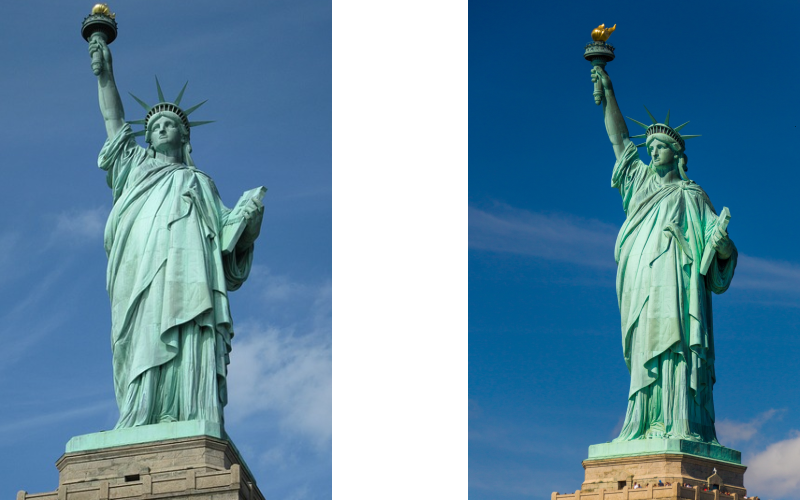
\includegraphics[scale=0.6]{images/liberty.png}
	\caption{Zwei Bilder mit dem gleichen Objekt aus unterschiedlicher Perspektive und in verschiedenen Lichtverhältnissen.}
	\label{img:liberty}
\end{figure}

Die Gewinnung der Features ist in die Schritte Detektion und Extraktion aufgeteilt: 

\begin{itemize}
	\item \textbf{Detektion} Ein Feature-Detektor in der Bildverarbeitung untersucht das Bild auf \enquote{interessante} Regionen. Die Definition hängt hier maßgeblich vom verwendeten Verfahren ab. Allgemein wird zwischen Detektoren unterschieden die Ecken, Kanten und Regionen betrachten. Einige der Detektoren berücksichtigen hier auch mehr als eine Kategorie: Das Difference of Gaussians Verfahren dient beispielsweise der Erkennung von Ecken und Regionen. Als Ergebnis liefert ein Detektor eine Menge von Pixel und ggf. ihrer Nachbarschaften. Diese Pixel sind die sogenannten \textit{keypoints} und beschreiben, mit ihren Nachbarschaften, die eingangs erwähnten \enquote{interessanten} Stellen.\newline
	 Um praktisch einsetzbar zu sein, muss ein Detektor ein Feature, dass in verschiedenen Bildern auftaucht, zuverlässig erkennen. Hier sollte aber die angestrebte Allgemeinheit berücksichtigt werden: Ein Feature Detektor für medizinische Bilder, z.B. Röntgenaufnahmen, kann speziellere Annahmen treffen, als einer für eine allgemeine Bildsuche. In Abbildung \ref{img:keypoints} sind die durch einen SIFT-Detektor gefundenen \textit{keypoints} farblich hervorgehoben.
	\item \textbf{Extraktion} Die Feature Extraktion erzeugt aus den vom Detektor gefundenen \textit{keypoints} und seinen lokalen Informationen den Deskriptor. Ein Feature-Deskriptor ist eine kompakte Darstellung eines Features. Die \textit{keypoints} und deren Nachbarschaften werden in Zahlen kodiert. Die meisten Deskriptoren kodieren die Informationen bereits normalisiert im Intervall zwischen 0 und 1. Diese Sequenz wird als ein Vektor notiert, sodass auch von Feature-Vektor gesprochen wird. Einige Verfahren reichern den Deskriptor mit zusätzlichen Informationen an, z.B. über die Stärke eines Gradienten bei der Kantendetektion.
\end{itemize}

\begin{figure}
	\centering
	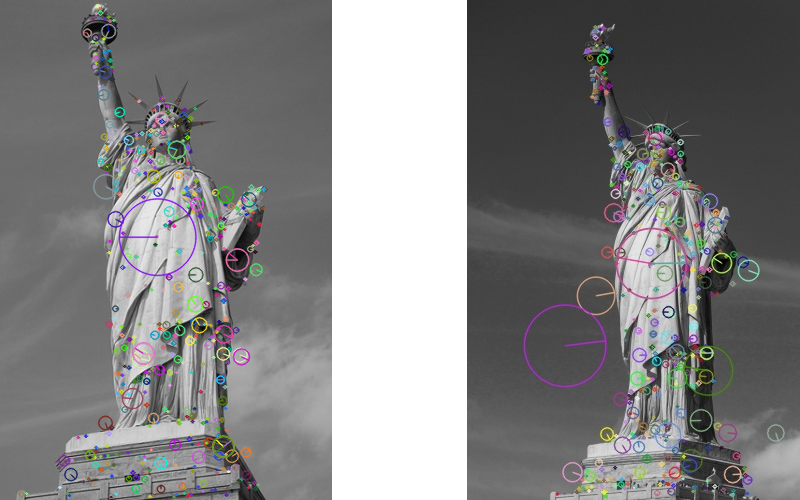
\includegraphics[scale=0.6]{images/liberty_kp.png}
	\caption{Gefundene \textit{keypoints} der beiden vorigen Bilder der Freiheitsstatuen farblich hervorgehoben (SIFT Detektor)}
	\label{img:keypoints}
\end{figure}

\subsection{Bildoperationen}

Zur Detektion und Extraktion von Features werden eine Reihe mathematischer Operationen und Verfahren genutzt, wie sie in der Bildverarbeitung üblich sind. Hiervon werden diejenigen vorgestellt, die im Weiteren in der Arbeit verwendet werden.

\subsubsection{Histogramm}

Ein Histogramm ist eine diskrete Funktion, welche die Häufigkeitsverteilung in einer Menge abbildet. Hierfür wird jeder Wert der Menge einer Klasse zugeordnet. Die Größe der Intervalle einer Klasse leiten sich aus der Größe des gesamten Wertebereichs ab. So kann beispielsweise die Verteilung der Pixel eines Bildes auf die Intensitäten als Histogramm betrachtet werden. Bei einem monochromatischen Bild liegen 256 Intensitätswerte vor, die je eine Klasse repräsentieren. Beim Bilden des Histogramms wird jeder Pixels betrachtet und der Zähler der Klasse um eins inkrementiert, in deren Wertebereich der Intensitätswert des Pixels fällt. Ein Histogramm ist normalisiert, wenn es die relative Verteilung in der Menge darstellt.
In Abbildung \ref{img:hist} sind im Wesentlichen zwei Bereiche zu erkennen: ein sehr heller Hintergrund und eine dunkle Katze, die den Großteil des Bildes ausmacht. Dies spiegelt sich auch im Histogramm wieder: Es ist eine große Mengen an Punkten im dunklen Bereich vorhanden (Intensität $< 128$) und eine kleine, extreme Häufung im hellen Bereich.

\begin{figure}
	\centering
	\includegraphics[scale=0.8]{images/big_cat.png}
	\caption{Graustufenbild und Verteilung der Intensitätswerte}
	\label{img:hist}
\end{figure}

\subsubsection{Filter} 
Ein Filter (auch Filterkern, Faltungsmatrix) ist eine, meist quadratische, Matrix von Koeffizienten. Eine Filteroperation auf einem Bild soll bestimmte Bestandteile, z.B. Rauschen, reduzieren oder andere Kanten bzw. Ecken hervorheben. Als Ergebnis dieses Prozesses resultiert also wieder ein Bild. Die Anwendung des Filters wird Faltung genannt und durch das $*$ Zeichen ausgedrückt. Hier handelt es sich aber nicht um eine klassische Matrixmultiplikation. Bei der Faltung wird zur Berechnung der neuen Intensität eines Pixels seine Nachbarschaft berücksichtigt. Bei Verwendung einer $3 \times 3$ Matrix zur Filterung bedeutet dies, dass der Pixel selbst und alle direkt angrenzenden, mit den entsprechenden Koeffizienten des Kerns multipliziert und anschließend aufsummiert werden. 

\textbf{Gauß-Filter}
Ein Gauß-Filter wird in der Bildbearbeitung verwendet um ein Bild zu verzerren und somit Rauschen aber auch Details zu unterdrücken. Diesem Filter liegt, wie der Name sagt, die Gauß-Funktion zu Grunde:

$$
g_{\sigma}(x)=\frac{1}{\sqrt{2\pi\sigma^{2}}}\mathrm{e}^{-\frac{x^{2}}{2\sigma^{2}}}, \quad g_{\sigma}(x, y) = \frac{1}{\sqrt{2\pi\sigma^{2}}}\mathrm{e}^{-\frac{x^{2} + y^{2}}{2\sigma^{2}}}
$$

Wird ein Gauß-Filter verwendet, so bedeutet dies, dass die Einträge der Matrix aus der Gauß-Funktion konstruiert sind. Für einen $3 \times 3$ Kernel mit einer Standardabweichung von $1.0$ ergibt sich folgende Matrix (Annäherung durch $1000$ Iterationen):

$$
\begin{bmatrix}
0.077847	& 0.123317	& 0.077847	\\
0.123317	& 0.195346	& 0.123317	\\
0.077847	& 0.123317	& 0.077847
\end{bmatrix}
$$ 

\textbf{Difference of Gaussians}
Durch den Difference of Gaussian (DoG) Operator können insbesondere Kanten hervorgehoben werden. Wie der Name andeutet wird hier die Differenz zwischen zwei Bildern gebildet, auf die jeweils ein Gauß-Filter angewandt wurde. Hier variieren die Standardabweichungen der Gauß-Funktionen um zwei unterschiedlich stark verzerrte Versionen des Originals $I$ zu erzeugen. Hierbei gilt, dass die Standardabweichung $\sigma_{2} > \sigma_{1}$ ist:

$$ DoG(x, y)_{\sigma_{1}, \sigma_{2}} = I * g_{\sigma_2}(x, y) - I * g_{\sigma_1}(x, y)$$

\subsection{Gradienten}

Ein Gradient beschreibt die Änderungen der Intensität eines Bildes in eine Richtung.  Ändert sich die Intensität beispielsweise proportional von Pixel zu Pixel, wird von einem linearen Gradienten gesprochen. In der Bildverarbeitung sind große bzw. plötzliche Änderungen in der Intensität von Bedeutung: Hier handelt es sich potentiell um Kanten, die für weitere Analysen des Bildes verwendet werden können. In Abbildung \ref{img:grad} ist links wieder das Bild der Freiheitsstatue dargestellt, rechts die berechneten Gradienten (Laplace Operator).

\begin{figure}
	\centering
	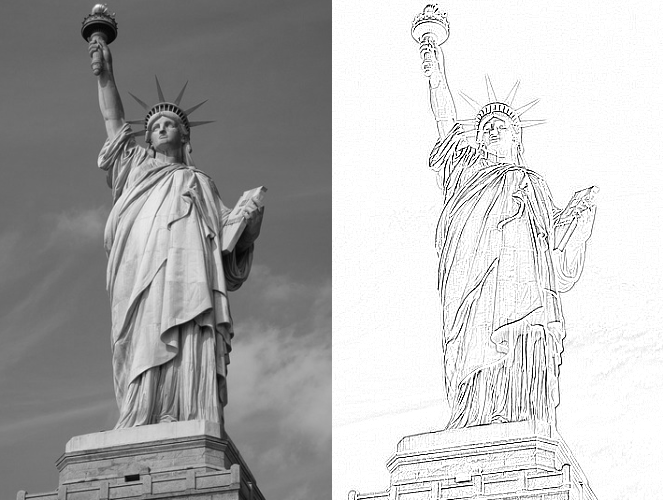
\includegraphics[scale=0.5]{images/liberty_grad.png}
	\caption{Links: Graustufenbild. Rechts: Ermittelte Gradienten eines Bildes in horizontale und vertikale Richtung.}
	\label{img:grad}
\end{figure}

\subsection{Histogram of Oriented Gradients}

Der Histogram of Orientied Gradients (HOG) Deskriptor beschreibt die Features als Histogramm der Richtung der Gradienten eines Bildes. Da sich Gradienten eignen, um Kanten in Bildern zu erkennen, wird so die Form der Objekte eines Bildes erkannt. Dalal und Triggs \cite{hog2005} entwickelten und nutzten diesen Verfahren bereits 2005, mit großem Erfolg, um Menschen in Bilder zu erkennen. 
Um ein HOG zu generieren, wird das Bild in gleich große Zellen eingeteilt, die eine Nachbarschaft von Pixeln umfassen. Über die Pixel jeder Zelle werden nun die lokalen Gradienten berechnet. Diese fließen proportional zu ihrer Stärke in den kumulierten Gradienten der Zelle ein. Dabei hat jede Zelle eine feste, vorgegebene Anzahl an Klassen für die Orientierungen der Gradienten. 
Dalal und Triggs nutzten in ihrer Originalarbeit als Fenster eine 64 $\times$ 128 Nachbarschaft von Pixeln, eine Zellgröße von 8 $\times$ 8 Pixeln und $2 \times 2$ Zellen pro Block. In Abbildung \ref{img:hog} ist links das Fenster dargestellt und rechts die entsprechenden Gradienten der Zellen. 

\begin{figure}
	\centering
	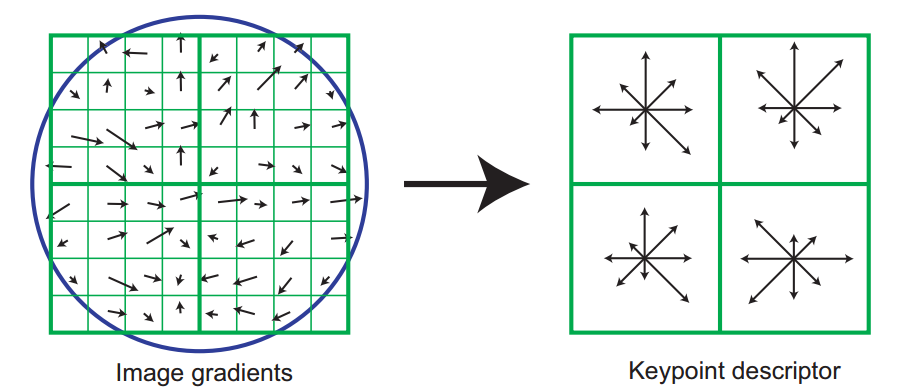
\includegraphics[scale=0.5]{images/hog.png}
	\caption{Schematische Darstellung des Histogram of Oriented Gradients  \cite{dif2004}}
	\label{img:hog}
\end{figure}

\subsection{SIFT}

SIFT ist ein Feature-Detektor und Deskriptor der 1999 von Lowe \cite{dif2004} entwickelt wurde. Neben der Größe bzw. den Maßstab, berücksichtigt SIFT teilweise auch die Rotation, Beleuchtung, Perspektive und Illumination. Der Algorithmus kombiniert mehrere mathematische Operationen und Verfahren um den Deskriptor eines Features als Ergebnis zu erhalten. Die Erzeugung des Deskriptors wird nach Lowe in vier wesentliche Schritte unterteilt:

\begin{enumerate}
	\item \textbf{Scale space} Im ersten Schritt wird der Maßstab behandelt. SIFT konstruiert hierfür einen \textit{scale space}. Hier werden aus dem Originalbild durch den \textit{Difference of Gaussians} immer verzerrtere Versionen erzeugt. Die Größe der neuen Bilder wird halbiert und die Prozedur wiederholt. Alle verzerrten Bilder einer Größe bilden eine sogenannte Oktave. SIFT verwendet vier Oktaven und fünf Bilder pro Oktave um den \textit{scale space} zu erzeugen. Um Ecken und Kanten in einem Bild zu ermitteln, die sich als Kandidaten für \textit{keypoints} eignen, wird nun zwischen allen aufeinanderfolgenden Bildern einer Oktave die Differenz gebildet. Das Prinzip ist für zwei Oktaven in Abbildung \ref{img:sift_dog} dargestellt. Das Ergebnis ist eine Approximation des \textit{Laplacian of Gaussians}\footnote{Der Laplacian of Gaussians (LoG) oder auch Marr-Hildreth-Operator dient ebenfalls der Kantendetektion in Bildern.}, jedoch ist dieses Verfahren weit weniger rechenintensiv. 

\begin{figure}
	\centering
	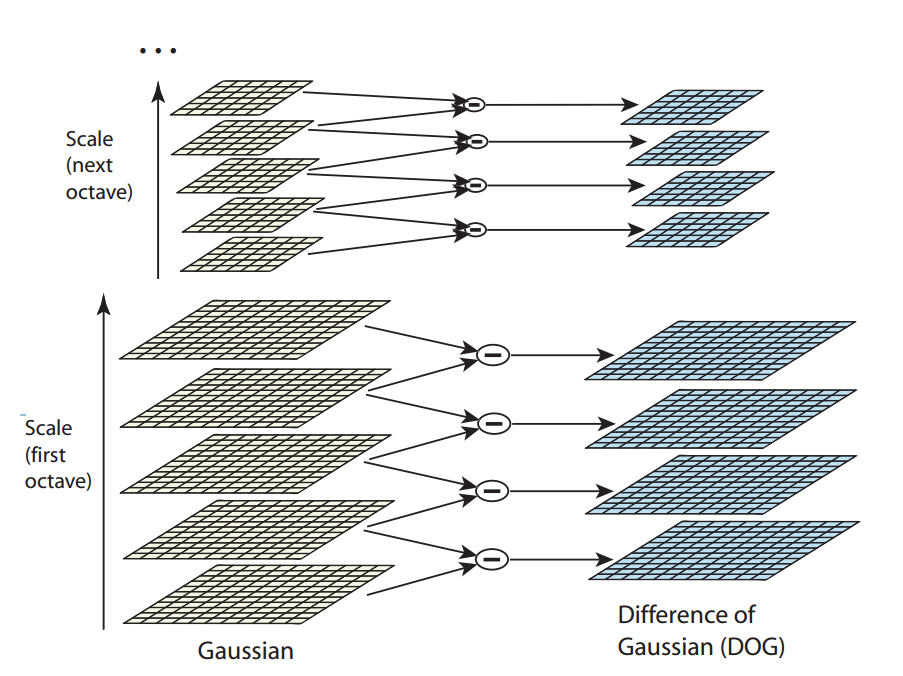
\includegraphics[scale=0.5]{images/sift_dog.png}
	\caption{Difference of Gaussians Operator \cite{dif2004}}
	\label{img:sift_dog}
\end{figure}	
	\item \textbf{Keypoint Ermittlung} Nicht alle Kandidaten werden zu \textit{keypoints}. Aus den DoG-Bildern werden nun die Extrempunkte bestimmt. Hierfür wird immer eine Nachbarschaft des DoG-Bildes und des Vorigen und Nachfolgenden im \textit{scale space} betrachtet. Da die Extremwerte nicht immer exakt auf einem Pixel liegen, muss die genaue Position noch berechnet werden. SIFT verwendet hierfür eine Taylor Entwicklung im angenäherten \textit{keypoint}.
	\item \textbf{Bestimmung der Orientierung} Bei dem Aufbau der Feature-Vektoren pro \textit{keypoint} wird die lokale Orientierung berechnet. Auf diese Weise sind die SIFT Deskriptoren invariant gegenüber Rotationen. Der SIFT Algorithmus berechnet ein Histogram of Oriented Gradients. Hierfür werden zufällig Punkte aus der Nachbarschaft des \textit{keypoints} ausgewählt. Das Maximum des Histogramms wird dann als dominante Orientierung verwendet.
	\item \textbf{Deskriptor} Für jeden durch den Detektor gefundenen \textit{keypoint} wird nun ein Feature-Vektor gebildet. Der Feature-Vektor enthält Informationen über die Nachbarschaft in Form der Gradienten. Das Fenster für die Auswahl der Nachbarschaft wird auf dem \textit{keypoint} zentriert und in vier Teilfenster unterteilt. Die Gradienten in allen Teilfenster werden in acht Richtungen gemessen, sodass der resultierende Deskriptor 128 Komponenten enthält.
\end{enumerate}

\section{Machine Learning}

\textit{Machine Learning} ist ein Teilgebiet der künstlichen Intelligenz und wird genutzt um Systeme zu entwerfen, die nicht explizit programmiert werden. Stattdessen lernen diese Systeme: Lernen bedeutet in diesem Kontext, dass ein System durch eine Eingabe seine Struktur verändert, um so die erwartete Leistung zu steigern. Dabei ist \textit{Machine Learning} ein interdisziplinäres Feld: Es sind sowohl Informatik, Statistik als auch biologische und kognitive Wissenschaften involviert. Bisher haben sich viele Anwendungsfälle für \textit{Machine Learning} Verfahren ergeben, die bis in den Alltag reichen. Einige Beispiele sind:

\begin{itemize}
	\item \textbf{Optical Character Recognition (OCR)} Unter OCR wird das Übersetzen eines (hand-)geschriebenen Textes in ein digitales Dokument bezeichnet. Beispielsweise kann so das Einfügen von Daten in CRM / ERP System automatisiert werden.
	\item \textbf{Spam Filterung} Das automatische Erkennen von unerwünschten E-Mails, die Werbung enthalten oder Betrugsversuche sind, ist inzwischen bei jedem Mail-Anbieter Teil des Angebots.
	\item \textbf{Spracherkennung} Auch eine Spracherkennung ist bereits auf den meisten digitalen Assistenten verfügbar und wird sogar zur Steuerung der häuslichen Elektronik verwendet.
	\item \textbf{Anomalie Erkennung} Digitale Geldtransaktionen werden heute von Algorithmen überwacht, die Abweichungen im Zahlungsverhalten beobachten. Wird eine ungewöhnlich hohe Summe überwiesen oder abgehoben, kann so informiert und auch interveniert werden.
\end{itemize}

All diese Verfahren nutzen eine große Menge an Trainingsdaten, um so ein Modell zu generieren, welches eine Klassifizierung weiterer Daten ermöglicht. Beispielsweise müssen bei einem System zur Spam-Filterung sowohl \enquote{normale} als auch Spam E-Mails verwendet werden, eine Spracherkennung benötigt digitale Aufnahmen von Wörtern und Sätzen zum Lernen, etc.
Nach dem Aufbau des Modells findet dann durch das System die Klassifizierung von Test- bzw. realen Daten statt. Es wird beispielsweise bei OCR entschieden, welches digitale Pendant zum vorliegenden Zeichen gehört oder bei der Spam-Filterung wie hoch die Wahrscheinlichkeit ist, dass es sich bei einer Mail um Spam handelt. Diese Trainings- und Testphase sind typisch für maschinelle Lernmethoden. Allgemein eignet sich solch ein Ansatz:

\begin{itemize}
	\item Um Beziehungen und Muster in den Daten zu entdecken, die nicht offensichtlich sind. Genau mit dieser Fragestellung beschäftigt sich die Disziplin des \textit{Data Mining}. Hierfür werden u.a. maschinelle Lernalgorithmen genutzt.
	\item Wenn kein klassischer Algorithmus für die Problemstellung entworfen werden kann oder das Programm zu komplex ist, als dass es von Menschen kodiert und gewartet werden könnte.
	\item Um neue Informationen einzubeziehen. Das Modell basiert auf den Daten, daher kann das System sich theoretisch durch neue Daten verändern und so der Situation anpassen.
\end{itemize}

\subsection{Lernverfahren}

Je nach Fragestellung haben sich unterschiedliche Methoden entwickelt, um den Lernprozess in einem System abzubilden. Im Wesentlichen werden drei Arten des maschinellen Lernens unterschieden:

\begin{itemize}
	\item \textbf{Überwachtes Lernen (supervised learning)} Ein überwachtes Lernverfahren soll eine Funktion $f$ lernen, die Eingaben ($x$) ihren Ausgaben ($y$) zuordnet, sodass gilt: $y = f(x)$ . Diese Funktion wird anhand von Trainingsdaten gelernt, die demzufolge aus Paaren von Eingaben und ihren dazugehörigen Ausgaben bestehen.
	\item \textbf{Unüberwachtes Lernen (unsupervised learning)} Ziel unüberwachter Lernalgorithmen ist es, großen Mengen von nicht kategorisierten Daten zu gruppieren oder zu komprimieren. Dadurch können Beziehungen in den Daten entdeckt bzw. kompaktere Darstellungen erreicht werden.
	\item \textbf{Verstärkendes Lernen (reinforcement learning)} Beim verstärkenden Lernen hat ein Agent die Aufgabe ein vorgegebenes Ziel zu erreichen, indem er mit seiner Umwelt agiert. Die Umwelt ist dabei eine Menge von Zuständen zwischen denen der Agent durch eine Aktion wechselt. Dabei hat jede Aktion eine Belohnung oder Bestrafung zufolge. Der Agent optimiert dann sein Verhalten, um die erhaltenen Belohnungen zu maximieren.
\end{itemize}

Beim überwachten Lernen ist es notwendig, dass sowohl Ursachen (Eingaben) als auch Effekte (Ausgaben) gemessen wurden. Hier sollen dann durch ein trainiertes Modell eine Vorhersage der Ausgabe abhängig von der Eingabe erfolgen. Beim unüberwachten Lernen hingegen sind die Eingaben latente Variablen. Das heißt, sie sind nicht direkt gemessen worden, sondern durch mathematische Verfahren von Observationen abgeleitet. Dadurch ist ein exploratives Vorgehen möglich. Es können Beziehungen in den Daten entdeckt und Gruppierungen bzw. Klassifizierungen durchgeführt werden.

\section{Autoencoder}

Durch den Aufschwung des maschinellen Lernens in den letzten Jahren sind neuronale Netze stark in den Fokus der Industrie und Wissenschaft gerückt. Solche künstlichen neuronalen Netze werden genutzt, um aus Beispielen Muster zu lernen und dieses Wissen zu transferieren. 
Ein spezielles neuronales Netzwerk zum unbeaufsichtigten Lernen ist der Autoencoder. Diese Art von Netzwerk lernt selbstständig eine komprimierte Darstellung der Eingabe. 
Als erstes wird im folgenden Abschnitt der Aufbau und die Funktionsweise eines Autoencoders erläutert. Darauf aufbauend werden zwei Erweiterungen des Autoencoders vorgestellt: Der Stacked Autoencoder und der Denoising Autoencoder. Ersterer wird verwendet, um effektiv tiefe Netzwerke zu konstruieren, letzterer ermöglicht eine korrekte Konstruktion aus verzerrten Daten.

\subsection{Neuronale Netze}

Neuronale Netze sind dem Aufbau und der Funktionsweise der Neuronen des menschlichen Gehirns nachempfunden. Es wird eine Menge von künstlichen Neuronen genutzt, um eine Lösung für ein Problem zu gestalten. Erste theoretische Überlegungen tauchten bereits in den 40er Jahren auf. Durch die wachsende Rechenleistung und neue Forschungsgebiete wie \textit{Machine Learning} finden neuronale Netze seit Mitte der 80er Jahre vermehrt praktische Anwendung und akademische Zuwendung \cite{nnk2007}. Dadurch, dass neuronale Netze von Natur aus hoch parallel arbeiten können, eignen sie sich vor allem für parallele Architekturen und die Verarbeitung großer Datenmengen. 

\subsubsection{Modell}
Ein neuronales Netz besteht aus einer Menge Neuronen, die in Schichten im Netzwerk angeordnet sind. Jedes Neuron besitzt einen Aktivierungszustand und einen Schwellwert. Von diesen hängt ab, ob ein Signal weitergeleitet wird. Neuronen benachbarter Schichten sind, meist vollständig, durch gewichtete Kanten miteinander verbunden. Diese Beziehung wird in einer Gewichtsmatrix ausgedrückt. Eine Kante zwischen zwei Neuronen die nicht verbunden sind, hat dann den Wert 0 als Gewicht, um die Abwesenheit auszudrücken. 
Das Netz verarbeitet ein Signal, welches hier als Vektor $x \in [0,1]^n$ aus $\mathbb{R}^n$ dargestellt wird. Die erste Schicht des Netzwerks, der \textit{Input Layer}, leitet das Signal nur an die nächste Schicht weiter und besitzt daher $n$ Neuronen. Die letzte Schicht, der \textit{Ouput Layer}, dient zur Ausgabe des Ergebnisvektors $z \in [0,1]^m$, wobei $m$ die Anzahl der Elemente des Vektors angibt. Zwischen diesen beiden Schichten können sich beliebig viele \textit{Hidden Layer} befinden. Die \textit{Hidden Layer} bilden somit den Kern des Netzes, deren Kantengewichtungen, Kanten oder Neuronen während eines Lernprozess angepasst werden können. \newline
In Abbildung \ref{img:nnexample} ist ein Netz mit drei Schichten dargestellt. Der \textit{Input Layer} nimmt einen Vektor mit vier Komponenten als Eingabe entgegen. Die Werte des Vektors werden an jedes der fünf Neuron im \textit{Hidden Layer} weitergeleitet, was durch die Kanten symbolisiert wird. Jede Kante besitzt dabei ein Gewicht, dass aus Gründen der Übersicht nicht aufgeführt ist. Schließlich werden die Ausgaben des \textit{Hidden Layers} an das einzige Neuron des \textit{Output Layers} geschickt und von diesem als Ergebnis $z$ ausgegeben.

\begin{figure}
	\centering

	\begin{tikzpicture}[shorten >=1pt,->,draw=black!50, node distance=\layersep]
    \tikzstyle{every pin edge}=[<-,shorten <=1pt]
    \tikzstyle{neuron}=[circle,fill=black!25,minimum size=17pt,inner sep=0pt]
    \tikzstyle{input neuron}=[neuron, fill=green!50];
    \tikzstyle{output neuron}=[neuron, fill=red!50];
    \tikzstyle{hidden neuron}=[neuron, fill=blue!50];
    \tikzstyle{annot} = [text width=6em, text centered]

    % Draw the input layer nodes
    \foreach \name / \y in {1,...,4}
        \node[input neuron, pin=left:$x_{\y}$] (I-\name) at (0,-\y) {};

    % Draw the hidden layer nodes
    \foreach \name / \y in {1,...,5}
        \path[yshift=0.5cm]
            node[hidden neuron] (H-\name) at (\layersep,-\y cm) {};

    % Draw the output layer node
    \node[output neuron,pin={[pin edge={->}]right:$z$}, right of=H-3] (O) {};

    % Connect every node in the input layer with every node in the
    % hidden layer.
    \foreach \source in {1,...,4}
        \foreach \dest in {1,...,5}
            \path (I-\source) edge (H-\dest);

    % Connect every node in the hidden layer with the output layer
    \foreach \source in {1,...,5}
        \path (H-\source) edge (O);

    % Annotate the layers
    \node[annot,above of=H-1, node distance=1cm] (hl) {Hidden Layer};
    \node[annot,left of=hl] {Input Layer};
    \node[annot,right of=hl] {Output Layer};
	\end{tikzpicture}

	\caption{Beispiel eines dreischichtigen neuronalen Netzes.}
	\label{img:nnexample}
\end{figure}

Die Verarbeitung eines Signals in einem Neuron ist in Abbildung \ref{img:neuron} schematisch dargestellt und lässt sich in drei Schritte untergliedern:
\begin{itemize}
	\item \textbf{Propagierungsfunktion} Aus der Eingabe aller verbundenen Neuronen wird die Netzeingabe $net_{in}$ berechnet. Meist wird hier die gewichtete Summe zwischen Eingabe und Gewicht verwendet: 
	$$net_{in} = \sum_{i=1}^{} w_{i}x_{i} + b$$
Die Variable $b$ ist hier der sogenannter Bias-Vektor, der dazu verwendet werden kann Einfluss auf die Aktivierung zu nehmen. Dieser wird als zusätzliches Neuron pro Schicht modelliert.
	\item \textbf{Aktivierungsfunktion} Es wird der neue Aktivierungszustand des Neurons aus dem alten Zustand und der Netzeingabe $net_{in}$ durch die Aktivierungsfunktion $a$ berechnet. Häufig wird hier die ReLU (Rectified Linear Unit) $a_{relu}$ bzw. die Sigmoidfunktion $a_{s}$ verwendet:
	$$a_{relu}(x) = \max(0,x) \quad \quad a_{s}(x) = \frac1{1+e^{-x}}$$
	\item \textbf{Ausgabefunktion} Wird ein Neuron aktiviert, so wird das resultierende Signal durch die Ausgabefunktion $net_{out}$ berechnet und an alle Neuronen in der folgenden Schicht weitergeleitet. Oft wird hier die Identitätsfunktion verwendet.
\end{itemize}

\begin{figure}
	\centering

	\begin{tikzpicture}[shorten >=1pt,->,draw=black!50, node distance=\layersepN]
    \tikzstyle{every pin edge}=[<-,shorten <=1pt]
    \tikzstyle{neuron}=[circle,fill=black!25,minimum size=27pt,inner sep=2pt]
    \tikzstyle{input neuron}=[neuron, fill=green!50];
    \tikzstyle{output neuron}=[neuron, fill=white!0];
    \tikzstyle{hidden neuron}=[draw, rectangle, minimum height=10mm, minimum width=10mm, fill=red!50];
    \tikzstyle{annot} = [text width=9em, text centered]

    % Draw the input layer nodes
    \node[input neuron, pin=left:$x_{1}$] (I-1) at (0,-1) {$w_{1}$};
	\node[input neuron, pin=left:$x_{2}$] (I-2) at (0,-2) {$w_{2}$};
    \node[input neuron, pin=left:$x_{n}$] (I-3) at (0,-3) {$w_{n}$};

    % Draw the sum
    \path[yshift=0.5cm]
    node[hidden neuron] (H-sum) at (\layersepN,-2.5cm) {$\sum$};

    % Draw the activation
    \path[yshift=0.5cm]
    node[hidden neuron] (H-act) at (\layersepN * 2,-2.5cm) {$s$};

    % Draw the output (invisible)
    \node[output neuron, right of=H-act] (O) {};

    % Connect input to sum
    \path (I-1) edge (H-sum);
    \path (I-2) edge (H-sum);
    \path (I-3) edge (H-sum);

	% Connect sum to act
    \path (H-sum) edge (H-act);

    % Connect act to output
    \path (H-act) edge (O);

    % Annotate the layers
    \node[annot,above of=H-sum, node distance=1.2cm] {Propagierungs-\\ funktion};
    \node[annot,above of=H-act, node distance=1.2cm] {Aktivierungs-\\ funktion};

	% Annotate edges
	\node[annot,above of=H-act, right=-0.3cm, node distance=0.2cm] {Aktivierung};
	\node[annot,above of=H-sum, right=-0.3cm, node distance=0.2cm] {Netzeingabe};
	
	\end{tikzpicture}

	\caption{Verarbeitung eines Signales in einem Neuron (ohne Ausgabefunktion).}
	\label{img:neuron}
\end{figure}

\subsubsection{Training und Lernprozess}

Wurde ein neuronales Netz konstruiert, folgt darauf die Trainingsphase. Durch das Training ist es möglich, dass ein Netzwerk Neuronen oder Verbindungen hinzufügt bzw. entfernt, den Schwellwert für die Aktivierung von Neuronen verändert oder die Gewichte zwischen Neuronen anpasst. Pro Trainingselement wird die Fehlerquote $F$ zwischen dem angestrebten Ergebnis $z'$ und der Ausgabe des Netzes $z$ berechnet:
$$ F(z, z')=\sum_{i=0}^{m}(z'_{i} - z_{i})^2 $$
Durch eine Lernregel werden abhängig von der Fehlerquote beispielsweise die Gewichte der Kanten angepasst. Für Netze ohne \textit{Hidden Layer} eignet sich hier die Hebbsche oder Delta Lernregel. Für Netze mit mindestens einem \textit{Hidden Layer}, hat sich das \textit{Backpropagation} Verfahren etabliert. \textit{Backpropagation} minimiert den Gradientenabstieg auf der Fehleroberfläche die $F$ aufspannt. Der Algorithmus geht in drei Schritten vor:

\begin{enumerate}
	\item \textbf{Forward Pass} Die Gewichte des Netzwerks werden initialisiert und eine Eingabe durch das Netz propagiert. Als Resultat liegt die Ausgabe vor.
	\item \textbf{Fehlerberechnung} Die Fehler des \textit{Output Layers} werden, durch einen Vergleich mit den erwarteten Werten, berechnet. Falls die Fehler unterhalb einer vorgegebenen Grenze liegen, ist das Training beendet. Andernfalls wird fortgefahren.
	\item \textbf{Backward Pass} In diesem Schritt wird die Fehlerquote rückwärts durch das Netz propagiert. Die Gewichte an den Verbindungen zwischen Neuronen werden in Abhängigkeit ihres Einflusses auf den Fehler Schicht für Schicht aktualisiert.
\end{enumerate}

\subsubsection{Hyperparameter}

Bisher wurde das Netzwerk und die Parameter, die es optimiert, die Gewichte $w$ und der Bias-Vektor $b$, betrachtet. Darüber hinaus gibt es eine Reihe von Parametern, die Hyperparameter, die vor Anwendung des Modells festgelegt werden müssen. Die wesentlichen Hyperparameter für neuronale Netze sollen hier vorgestellt und ihr Einfluss auf das Modell erläutert werden. Die aufgeführten Standardwerte wurden bei einer Vielzahl von Modellen beobachtet, gelten aber nicht uneingeschränkt für jeden Anwendungsfall \cite{pda2012}. 
%https://arxiv.org/pdf/1206.5533.pdf

\textbf{Initiale Lernrate} Bei gradientenbasierten Verfahren wird in jeder Iteration der Fehler zurückpropagiert. Dies wird in den meisten Fällen zu einer zu schnellen Anpassung des Netzes führen und es \enquote{vergisst} schnell, was es bereits gelernt hat. Aus diesem Grund werden die berechneten Fehler mit der Lernrate (\textit{learning rate}), einem kleinen Wert, multipliziert. Praktisch wird für die Lernrate ein Wert kleiner 1 und größer $10^{-6}$ verwendet.\newline

\textbf{Anzahl der Trainingsiterationen} Eine Iteration entspricht einem \textit{forward} und \textit{backward pass} einer kleinen Teilmenge (ein \textit{batch}) der gesamten Trainingsmenge. Eine zu große Anzahl an Iterationen führt zu einer Überanpassung des Netzes an die Trainingsdaten, daher sollte gestoppt werden, wenn sich andere Metriken nicht mehr verbessern.\newline

\textbf{Anzahl der Exemplare pro Trainingsiteration} (\textit{batch size)} Je größer die \textit{batch size}, desto mehr Trainingsexemplare werden pro Iteration verarbeitet. Durch einen größeren Wert kann die Berechnung beschleunigt werden, allerdings ist auch mehr Speicher erforderlich. In der Praxis liegt der Wert für diesen Parameter meist zwischen 16 und 128 (Zweierpotenzen). 

\subsection{Aufbau und Funktionsweise}

Ein Autoencoder (AE) ist ein spezielles neuronales Netzwerk, das eine komprimierte Kodierung der Eingabe lernt. Diese Art von Netzwerk versucht, die Daten zu rekonstruieren und kann daher unbeaufsichtigt lernen: Die rekonstruierten Daten können anhand einer Distanzmetrik mit den Originaldaten verglichen werden. Anschließend kann die Größe des Fehlers berechnet werden und durch \textit{Backpropagation} die Gewichtmatrix aktualisiert werden \cite{ssn1997}.
Um die Originaldaten als Ergebnis erhalten zu können, muss die Anzahl der Neuronen des \textit{Input Layers} der Anzahl der Neuronen im \textit{Output Layer} entsprechen. Die Anzahl der Neuronen im \textit{Hidden Layer} ist geringer, um die komprimierte Darstellung des Features zu erreichen. Werden mehrere \textit{Hidden Layer} verwendet, so nimmt die Neuronenanzahl von Schicht zu Schicht ab um die Anzahl der Komponenten weiter zu verringern. Dieser Vorgang ist die Enkodierung und liefert die gewünschte komprimierte Abbildung. Die Dekodierung ist umgekehrt aufgebaut, um das Original aus der komprimierten Repräsentation Schicht für Schicht zu rekonstruieren. Wie gut die Dekodierung gelungen ist, lässt sich dann anhand eines Vergleichs der Distanz des Original und der Rekonstruktion bewerten.\newline
Formal wird ein Eingabevektor $x \in [0,1]^n$ auf einen Vektor $y \in [0,1]^p$, mit $p < n$, abgebildet: 
$$y = encode_{W,b}(x) = s(Wx + b)$$
$W$ ist die Gewichtsmatrix der Größe $n \times p$ und $b$ der Bias-Vektor. Diese Parameter werden durch den Autoencoder optimiert. Die Darstellung $y$ wird in diesem Kontext auch als \textit{code} bzw. latente Variablen bezeichnet. Die Rekonstruktion erfolgt durch die Dekodierungsfunktion. Der Vektor $z \in [0, 1]^n$ berechnet sich durch: 
$$z = decode_{W', b'}(y) = s(W'y + b')$$
In Abbildung \ref{img:example_ae} ist ein Autoencoder abgebildet, der als Eingabe einen Vektor $x \in [0,1]^4$ entgegen nimmt. Dieser wird auf den Vektor $y$ mit drei Komponenten abbildet, da der \textit{Hidden Layer} drei Neuronen enthält. Die Rekonstruktion $z$ aus $y$ erfolgt dann durch die Berechnung der Dekodierungsfunktion.

\begin{figure}
	\centering

	\begin{tikzpicture}[shorten >=1pt,->,draw=black!50, node distance=\layersep]
    \tikzstyle{every pin edge}=[<-,shorten <=1pt]
    \tikzstyle{neuron}=[circle,fill=black!25,minimum size=17pt,inner sep=0pt]
    \tikzstyle{input neuron}=[neuron, fill=green!50];
    \tikzstyle{output neuron}=[neuron, fill=red!50];
    \tikzstyle{hidden neuron}=[neuron, fill=blue!50];
    \tikzstyle{annot} = [text width=6em, text centered]

    % Draw the input layer nodes
    \foreach \name / \y in {1,...,4}
        \node[input neuron, pin=left:$x_{\y}$] (I-\name) at (0,-\y) {};

    % Draw the hidden layer nodes
    \foreach \name / \y in {1,2,3}
        \path[yshift=-0.5cm]
            node[hidden neuron] (H-\name) at (\layersep,-\y cm) {$y_{\y}$};
    
    % Draw the output layer nodes
    \foreach \name / \y in {1,...,4}
        \node[output neuron,pin={[pin edge={->}]right:$z_{\y}$}, right of=H-3] (O-\name) at (\layersep,-\y) {};

    % Connect every node in the input layer with every node in the
    % hidden layer.
    \foreach \source in {1,...,4}
        \foreach \dest in {1,2,3}
            \path (I-\source) edge (H-\dest);

    % Connect every node in the hidden layer with the output layer
    \foreach \source in {1,2,3}
        \foreach \dest in {1,...,4}
        	\path (H-\source) edge (O-\dest);

    % Annotate the layers
    \node[annot,above of=H-1, node distance=1.5cm] (hl) {Hidden Layer};
    \node[annot,left of=hl] {Input Layer};
    \node[annot,right of=hl] {Output Layer};
	\end{tikzpicture}

	\caption{Beispiel eines simplen Autoencoders}
	\label{img:example_ae}
\end{figure}

\subsection{Stacked Denoising Autoencoder}

Von Hinton and Salakhutdinov wurde 2006 \cite{dae2006} das Konzept des Stacked Autoencoders eingeführt, um einige Probleme mit herkömmlichen Autoencoder zu überwinden. Bei Netzwerken mit mehr als einem \textit{Hidden Layer} erzielt die Methode des steilsten Abstiegs, aufgrund der zunehmenden Verzerrung der Gradienten, bei der Rückpropagierung keine guten Ergebnisse mehr. In vielen Ansätzen wurde auch eine zufällige Initialisierung der Gewichte gewählt. Hier besteht die Gefahr, dass der Algorithmus in einem lokalen Optimum verbleibt. Wenn die anfänglichen Gewichte hingegen bereits nah an einer guten Lösung liegen, sinkt die Wahrscheinlichkeit eines lokalen Optimums. Aus diesem Grund wurde das Pretraining für Autoencoder mit mehr als einer Schicht vorgeschlagen. In diesem Training wird jedes Paar aneinanderliegender Schichten als ein Autoencoder aufgefasst und einzeln trainiert. Das Pretraining besteht aus drei Schritten, die wiederholt werden, bis alle Autoencoder trainiert sind.

\begin{enumerate}
	\item Es wird der aktuelle Autoencoder trainiert. Zu Beginn besteht dieser aus dem \textit{Input} und folgendem \textit{Hidden Layer}.
	\item Nun wird der Decoder des trainierten Autoencoders entfernt und ein neuer Autoencoder erzeugt. Dieser besitzt den \textit{Hidden Layer} des trainierten Autoencoders als \textit{Input Layer}.
	\item Das Training wird mit dem neuen Autoencoder fortgeführt.
\end{enumerate}

Ein Denoising Autoencoder \cite{sda2010} dient dazu, eine korrumpierte Eingabe zu korrigieren. Die Korruption ist hier als Rauschen bzw. Verzerrung (\textit{noise}) aufzufassen. In vielen Arten von Features, z.B. Bildern oder Audiomaterial, sind Verzerrungen bereits in den Daten vorhanden, beeinflussen die Semantik des Ganzen aber kaum. Daher soll der Autoencoder dies bereits berücksichtigen, indem er nicht direkt mit der Eingabe $x$ arbeitet. Stattdessen wird $x$ auf die korrumpierte Eingabe $\widetilde{x}$ durch ein stochastisches Verfahren abgebildet. In der Enkodierungsfunktion wird dann $\widetilde{x}$ statt $x$ verwendet: 
$$encode_{W,b}(\widetilde{x}) = s(W\widetilde{x} + b)$$
In der Praxis hat sich zur Korruption der Eingabe die \textit{masking corruption} Technik bewährt: Hierbei werden 20\% bis 50\% der Neuronen des \textit{Input Layers} zufällige ausgewählt und werden \enquote{genullt}. Auf diese Weise wird vermieden, dass der Autoencoder nur von bestimmten Teilmengen an Neuronen abhängt  \cite{pda2012}.

\section{Bag of Visual Words}

Das Bag of Visual Words lehnt sich an das Bag of Words Modell aus dem Bereich Information Retrival an. Daher soll zunächst die Funktionsweise des Bag of Word Modells erläutert werden, um darauf aufbauend den Bag of Visual Words einzuführen.\newline 
Der Bag of Words wird zur Klassifizierung von Dokumenten genutzt. Dieses Verfahren zählt das Auftreten jedes Wortes in einem Dokument. Diese Anzahl wird durch die Anzahl aller Wörter im Vokabular dividiert, um die relative Häufigkeit eines Wortes zu ermitteln. Das Vokabular wird in diesem Kontext \textit{Codebook} genannt, die Wörter werden auch als \textit{Codewords} bezeichnet.\newline
Dieses Modell wurde von der digitalen Bildverarbeitung adaptiert \cite{bok2004}. Es wird anhand der Features von Trainingsbildern ein visuelles Vokabular gelernt, das zur Klassifizierung von Bildern dient. Die Features können aber nicht direkt statt der Worthäufigkeit verwendet werden: Ein Wort ist ein diskreter Wert, der direkt verglichen werden kann, \todo{ein Feature hingegen ist ein Vektor in einem hochdimensionalen Raum, der Eigenschaften beschreibt}\footnote{Neh. Hier floats statt int string}. Um konkrete Werte zu erhalten, ist es notwendig, die Vektoren zu quantisieren. Die quantisierten Vektoren entsprechen dann den \textit{Codewords} und werden in diesem Kontext auch \textit{Visual Words} genannt. \newline
Zunächst wird die Funktionsweise des Bag of Visual Words im folgenden Abschnitt näher betrachtet. Dem schließt eine Betrachtung des Kernstücks des Algorithms an: Das Clustering der Features. Hier wird ein k-means Algorithmus, Llyods heuristische Variante, verwendet. Es wird eine gängige sequentielle Implementierung angeführt, auf deren Basis dann die Parallelisierbarkeit durch Grafikkarten untersucht wird.\newline
Bei der Einordnung eines Bildes wird ein Histogramm der Visual Words generiert, daher wird im Anschluss ein sequentieller Histogramm Algorithmus vorgestellt, der auf Parallelisierbarkeit geprüft wird.

\subsection{K-means Clustering}

Unter k-means Clustering werden Algorithmen zusammengefasst, die eine Menge Vektoren durch Zuweisung in $k$ vorgegebene Gruppen einteilen, die sogenannten Cluster. Aus den Vektoren werden initial $k$ Stück ausgewählt, die als anfängliche Schwerpunkte der Cluster dienen. Ein k-means-Algorithmus ordnet nun iterativ jeden Vektor dem Cluster zu, der ihm am nächsten ist. Formal werden $n$ Vektoren aus dem Raum $\mathbb{R}^{d}$ in $k$ Cluster eingeteilt. $D$ ist hierbei eine Distanzmetrik im euklidischen Raum. Oft wird hier der quadrierte Fehler durch k-means minimiert, also beispielsweise $D = \|x_{i} - c_{j}\|^{2}$. Jeder Vektor $x_{i}$ wird dem Cluster $c_{j}$ zugeordnet, dessen Distanz zum Vektor am Geringsten ist:

$$ C(x_i) = arg \min_{j = 0,...,k} D(x_i, c_j) \quad i = 0,...,n$$

Soll ein globales Optimum gefunden werden, so ist k-means NP-schwer. Praktische Implementierungen approximieren daher meist die Schwerpunkte der Cluster, wie beispielsweise der Algorithmus von Llyod. Llyods Algorithmus beginnt mit einer Initialisierung der Schwerpunkte. Schritt zwei und drei werden dann solange wiederholt, bis der Algorithmus konvergiert, also die Vektor-Cluster-Zuordnung sich nicht mehr bzw. nur noch gering ändert oder eine maximale Anzahl an Iterationen erreicht wurde: 

\begin{enumerate}
	\item \textbf{Initialisierung} Es werden zunächst $k$ Vektoren durch ein Verfahren (z.B. zufällig oder \textit{farthest-neighbour}) als Schwerpunkte der Cluster ausgewählt.
	\item \textbf{Zuordnung}: Von den verbleibenden Vektoren wird nun mit jedem Clusterschwerpunkt die neue Summe der Varianzen bei Aufnahme des Vektors berechnet. Es wird der Vektor dem Cluster zugeordnet, dessen Varianz sich am Geringsten bei Aufnahme des Vektors erhöht.
	\item \textbf{Vektoren zuweisen}: Die Zentren der Cluster werden neu berechnet, um die neue Zuordnung der Vektoren zu Clustern in Folgeberechnungen miteinzubeziehen.
\end{enumerate}

Zur geometrischen Veranschaulichung sind in Abbildung \ref{img:kmeans} Punkte im zweidimensionalen Raum gegeben. Die Verteilung der Punkte ist in diesem Beispiel idealisiert, um bei einem Clustering mit einem $k = 3$, die Cluster in der rechten Grafik zu erhalten. Dies illustriert auch, dass abhängig von den Daten nicht immer sinvolle Cluster gebildet werden können. Die Wahl der initialen Clusterschwerpunkte kann das Ergebnis ebenfalls stark beeinflussen, daher sollte diese nicht immer zufällig gewählt werden. Beispielsweise wählt die \textit{farthest neighbour} Methode als initial Zentren die Vektoren, welche am weitesten voneinander entfernt sind \cite{mmd2011}.

\begin{figure}
	\centering
	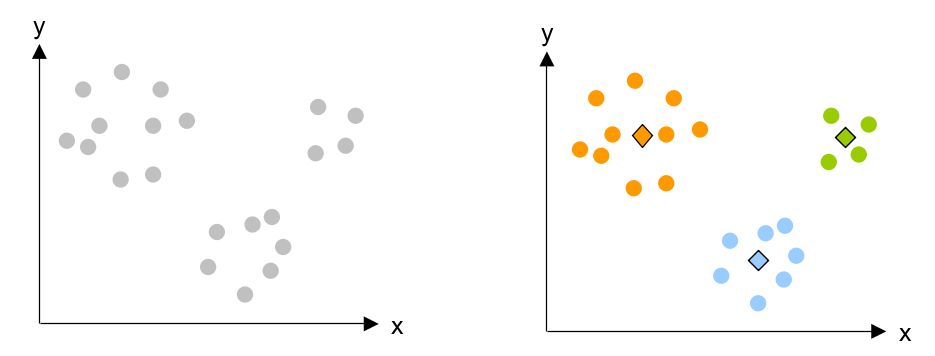
\includegraphics[scale=0.55]{images/kmeans.png}
	\caption{K-means Clustering im zweidimensionalen Raum mit $k = 3$.}
	\label{img:kmeans}
\end{figure}

\subsection{Funktionsweise}

Der Bag of Visual Words besteht aus einer Trainings- und Testphase, wie in Abbildung \ref{img:bovw} dargestellt. Die Extraktion der Features ist beiden Phasen vorgelagert.\newline
Zu Beginn erfolgt die Trainingsphase, das Clustering der extrahierten Features. Das so erzeugte \textit{Codebook} ist das Modell, gegen das anschließend getestet werden kann. Die Idee ist, dass ähnliche Feature-Vektoren nah beieinander im Raum liegen und somit in die gleiche semantische Kategorie gehören. Durch einen Clustering-Algorithmus wie k-means kann die Größe des \textit{Codebooks} bestimmt werden. Wird für $k$ eine große Zahl gewählt, wird ein Vokabular von Exemplaren aufgebaut, ein kleines $k$ hingegen erkennt eher Kategorien. Die Schwerpunkte der Cluster vertreten dann eine Menge von ähnlichen Features und bilden das \textit{Codebook} bzw. Modell.\newline
Der Testprozess erzeugt nun, auf Basis des \textit{Codebooks}, die \textit{Visual Words} von Bildern. Hierfür werden die Features eines Bildes extrahiert und ein Histogrammalgorithmus ermittelt die Verteilung der \text{Visual Words}: Für jedes Feature wird das ähnlichste \textit{Visual Word} des \textit{Codebooks} bestimmt und die entsprechende Klasse inkrementiert. Wird dieser Prozess auf zwei Bilder angewendet, so können die resultierenden Histogramme miteinander verglichen werden (z.B. mit dem \textit{MSE (mean squared error)} als Metrik).

\begin{figure}
	\centering
	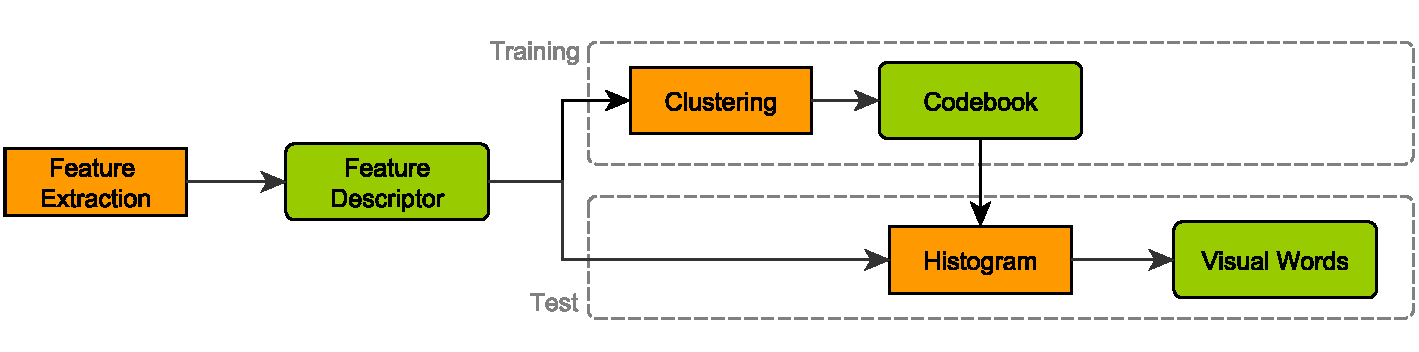
\includegraphics[scale=0.65]{images/bovw_process.pdf}
	\caption{Training- und Testprozess des Bag of Visual Word Modells.}
	\label{img:bovw}
\end{figure}

\subsection{Lloyds Algorithmus}

Im Grundlagenkapitel wurde bereits Lloyds Algorithmus eingeführt, hier soll zunächst näher auf die sequentielle Ausführung eingegangen werden, um anschließend eine mögliche Parallelisierung zu diskutieren. Im nachfolgenden Codelisting ist der Ablauf des Algorithmus in Pseudocode beschrieben. Als Parameter werden die Punkte $P$ und die Anzahl der zu bildenden Cluster $k$ erwartet. In Zeile 2 findet die Auswahl der initialen Schwerpunkte der Cluster statt. Die Zuordnung von Punkten zu Clustern erfolgt in Zeile 7: $argminD$ wählt den Cluster aus, dessen Varianz am Wenigsten bei Aufnahme des Punktes $p_{i}$ steigt. Abschließend wird die Aktualisierung der Schwerpunkte aller Cluster in der Schleife in Zeile 8 und 9 durchgeführt. \todo{Lol neu}

\lstset{language=C}
\begin{lstlisting}[mathescape=true]
kmeans_lloyd ($P, C, k$)
	initialisierung
	until convergence
		$C_{j} = 0, j = 1, ..., k$
		for each $p \in P$
			for each $c \in C$
				$c_{j} = argminD(c_{j}, p_{i})$		
		for each $c_{j} \in  C$
			$c = \frac{1}{|c|} \sum_{n \in c} n$
\end{lstlisting}

Die Initialisierungsphase muss für die Parallelisierung nicht beachtet werden: Sie nimmt nur wenig Zeit in Anspruch und wird einmalig zu Beginn ausgeführt. Die anderen beiden Schritte des Algorithmus bergen mehr Potential: In Zeile 5 bis 7 wird die Varianz jedes Cluster-Vektor Paares berechnet. Da die Berechnung der Varianz eines Paares unabhängig von der eines anderen ist, kann die Berechnung aller Varianzen parallel erfolgen. Nachdem für einen Durchgang die Veränderung der Mitgliedschaft von Vektoren zu Clustern berechnet wurde, müssen die Cluster-Schwerpunkte aktualisiert werden. Auch die Berechnung der neuen Schwerpunkte der Cluster kann unabhängig voneinander erfolgen: Die Vektoren aus denen der Mittelwert berechnet wird, sind genau einem Cluster zugeordnet.

% http://www.know-center.tugraz.at/download\_extern/papers/latex8.pdf

\subsection{Histogramme}

Ein sequentielles Histogramm kann als Programm in einer Schleife über die Daten ausgedrückt werden: Für jedes Element wird der Index der Klasse des Histogramms berechnet und um eins inkrementiert. Zur Normalisierung des Histogramms ist es anschließend notwendig, jede Klasse des Histogramms durch die Gesamtanzahl der Werte zu dividieren. Da es sich bei der Anzahl der Klassen jedoch um eine kleine Zahl, im Vergleich zur Anzahl der Elemente in den Daten, handelt, ist dieser Aufwand vernachlässigbar.
Um das Histogramm der Visual Words eines Bildes zu erzeugen, muss für jedes extrahierte Feature das nächste Visual Word bestimmt werden. Dies entspricht im nachfolgenden Pseudocode der doppelten Schleife über die Features $F$ und Cluster $C$ in Zeile 2 und 3. Der Index des nächsten Clusters wird dann in Zeile 4 durch $argmin D$ berechnet und in der nächsten Zeile wird das Histogramm $H$ an der entsprechenden Stelle inkrementiert.

\begin{lstlisting}[mathescape=true]
histogram ($P, C, H, k$)
	for each $p \in P$
		for each $c \in C$
			$bin = arminD(c, p)$ 
		$H_{k} = H_{k} + 1$		
	for each $h in H$
		$h = h / |H|$
\end{lstlisting}

\section{CUDA}

Der Begriff CUDA ist ein Akronym für \textit{Compute Unified Device Architecture}. Dahinter verbirgt sich eine Architektur von Nvidia für parallele Berechnungen durch Grafikkarten. Durch den Einsatz von Grafikkarten können Berechnungen gerade bei großen Datenmengen stark beschleunigt werden, da diese auf eine hoch-parallele Verarbeitung ausgelegt sind. Die meisten GPU Computing Ansätze, und auch CUDA, verwenden als Ausführungsmodell das Single Program Multiple Data (SPMD) Modell. Im Unterschied zum Multiple Instruction Multiple Data (MIMD) Modell, dass in CPUs verwendet wird, wenden alle Prozessoren das gleiche Programm auf unterschiedliche Daten an. Durch diese Art der Parallelisierung konnten in den letzten Jahren enorme Steigerungen der Gleitkommaoperationen pro Sekunde (flops) und der Speicherbandbreite bei Berechnungen erzielt werden.\newline
Der Abschnitt gibt im Wesentlichen ein Einblick in die im CUDA C Programming Guide \cite{cud2012} detailliert beschriebenen Dokumentation gegeben, sodass ein Leser Teile eines CUDA Programms nachvollziehen kann. Zunächst wird näher auf das Ausführungsmodell und dessen Umsetzung eingegangen. CUDA unterscheidet zwischen verschiedenen Speicherbereichen auf der Grafikkarte. Da die Verwendung der unterschiedlichen Speicherbereiche wesentliche Unterschiede in der Implementierung eines Algorithmus und dessen Laufzeit zur Folge hat, werden diese im Abschnitt \ref{cudaMemory} Speicherverwaltung behandelt. Um den praktische Einsatz von CUDA zu illustrieren, wird abschließend ein Programm zur Addition zweier Vektoren auf der Grafikkarte vorgestellt.

\subsection{Ausführungsmodell}

Ein Programm, das auf einer Nvidia Grafikkarte ausgeführt werden soll, muss in der Sprache CUDA C geschrieben sein. Aus der Sicht eines Programmierers handelt es sich hierbei um eine Erweiterung von C um Primitive und Funktionen für Berechnungen auf der Grafikkarte. Zum Übersetzen und Linken des Codes dient der \textit{nvcc} Compiler von Nvidia. Dieser unterscheidet zwischen Code der auf dem \textit{host}, der CPU, und dem \textit{device}, der GPU, ausgeführt wird. Das Kompilieren von \textit{host} Code erfolgt durch den auf dem \textit{host} installierten C Compiler. Der \textit{device} Code wird durch \textit{nvcc} zu \textit{PTX}\footnote{PTX steht für Parallel Thread eXecution und ist eine \enquote{zwischen} Assemblersprache. Der generierte Code ist noch nicht ganz optimiert, da PTX als Basis mehrerer GPU Generationen dient.} bzw. \textit{cubin binary code}\footnote{cubin Dateien sind gerätespezifische Binärdateien} übersetzt.
Nvidia hat das SPMD Modell durch \textit{kernels} umgesetzt. Ein \textit{kernel} ist ein Programm, das parallel auf verschiedene Daten der GPU angewendet wird. 
Bevor ein \textit{kernel} aufgerufen werden kann, muss der notwendige Speicher auf der Grafikkarte für die Daten und das Ergebnis allokiert werden. Anschließend werden die Daten von \textit{host} zu \textit{device} kopiert. Nach Durchführung der Berechnung kann dann das Ergebnis zurück zum \textit{host} kopiert werden. Die Datentransfers weisen eine nicht unbeachtliche Latenz auf. Folglich sollte das Kopieren von Daten nur selten erfolgen.\newline
Die Daten liegen in der Regel als Vektor oder Matrix vor. Der Zugriff auf verschiedene Elemente durch unterschiedliche \textit{kernel} erfolgt dann durch eine Indexberechnung. Diese wird anhand des Beispiels der Vektoraddition näher erläutert.\newline
CUDA erfordert, dass ein Programmierer die Größe bzw. Anzahl von Grids und Blocks festlegt. Ein Block ist eine logische Einheit und entspricht einem Multiprozessor der Grafikkarte. Durch diese Strukturierung können die Blöcke parallel auf der Hardware ausgeführt werden. Das Grid enthält die Blöcke und kann ein, zwei oder dreidimensional sein. Beim Aufruf des \textit{kernels} muss die Anzahl der Threads pro Block und die Anzahl der Blocks in einem Grid angegeben werden. In Abbildung \ref{img:cuda1} ist ein zweidimensionales Grid mit sechs zweidimensionalen Blöcken á 12 Threads schematisch dargestellt. Ein Block kann auf aktuellen Grafikkarten bis zu 1024 Threads beinhalten.

\begin{figure}
	\centering
	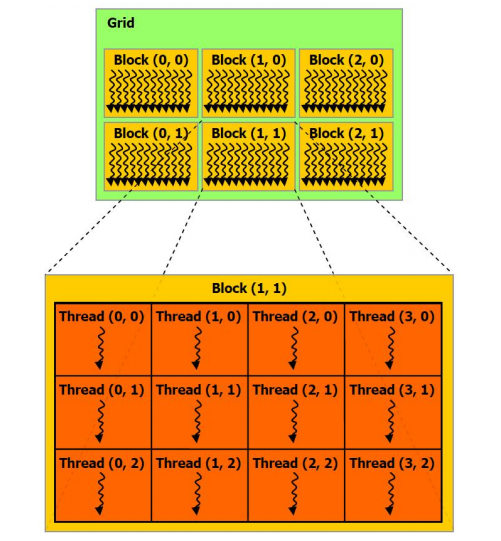
\includegraphics[scale=0.55]{images/cuda1.png}
	\caption{Organisierung von Threads in Blocks in Grids \cite{cud2012}}
	\label{img:cuda1}
\end{figure}

\subsection{Speicherverwaltung}
\label{cudaMemory}

Dadurch, dass die Daten vom \textit{host} zum \textit{device} kopiert werden müssen und vice versa, unterscheidet CUDA zwischen \textit{host memory} und \textit{device memory}. Darüber hinaus ist der \textit{device memory} bereits auf der Grafikkarte in verschiedene Bereiche organisiert, wie in Abbildung \ref{img:cuda_mem} dargestellt. Jeder Multiprozessor hat Zugriff auf den \textit{global memory} sowie einen eigenen lokalen \textit{shared memory}, \textit{constant} und \textit{texture cache}. Lokal erstellte Variablen werden als \textit{register} bezeichnet. Auf diese ist der Zugriff mitunter am schnellsten, jedoch sind sie lokal pro Thread. Die Daten liegen als Parameter zunächst im \textit{global memory} vor. Im \textit{constant cache} liegen alle durch das CUDA Schlüsselwort \textit{\textunderscore\textunderscore constant\textunderscore\textunderscore} deklarierte Werte. Zugriffe auf den \textit{global memory} sind am langsamsten, da der Speicherbereich zwischen allen Multiprozessoren geteilt wird und Zugriffe mitunter synchronisiert werden müssen. Durch Verwendung des \textit{shared memory} und \textit{texture cache} können Speicherzugriffe beschleunigt werden, jedoch können Daten aus diesen Bereichen nicht zwischen Blöcken geteilt werden.

\begin{figure}
	\centering
	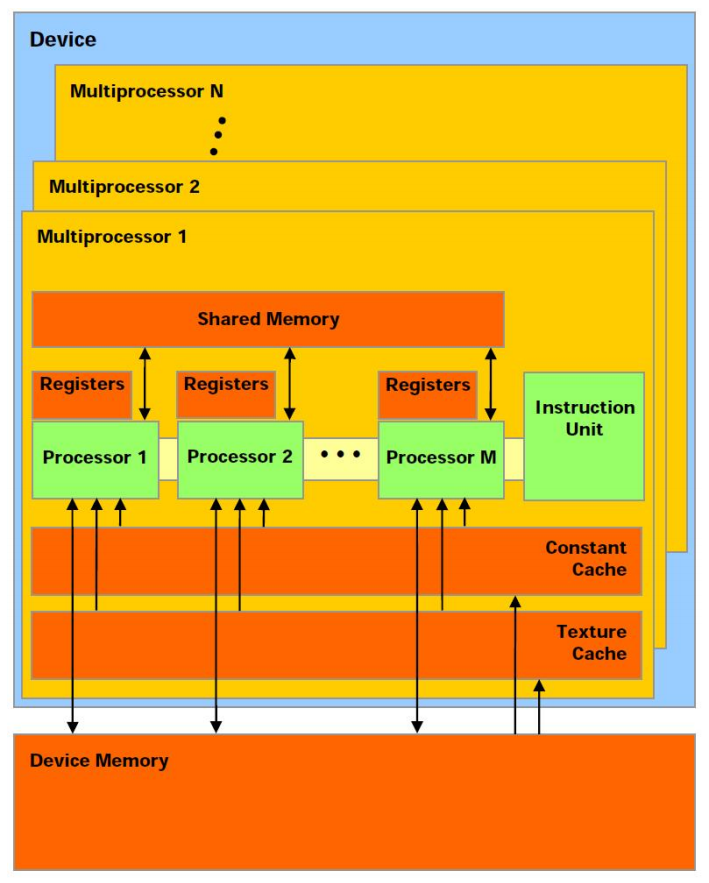
\includegraphics[scale=0.4]{images/cuda_mem.png}
	\caption{Organisierung der verschiedenen Speichertypen}
	\label{img:cuda_mem}
\end{figure}

\subsubsection{Shared Memory}

Gerade bei vielen parallelen Lese- / Schreibzugriffen kann hier eine hohe Latenz auftreten, wenn viele Threads auf die gleichen Adressen zugreifen. Aus diesem Grund empfiehlt es sich, die benötigten Daten von dem \textit{global} in den \textit{shared memory} zu kopieren. Der \textit{shared memory} wird von allen Threads in einem Block geteilt. Beim Kopieren der Daten muss ein Index berechnet werden, um die korrekten Daten dem jeweiligen Block zuzuordnen. Soll beispielsweise jeder \textit{kernel} auf dem Element eines Vektors arbeiten, setzt sich der globale Index aus der Position im Block und im Thread zusammen: $blockDim.x * blockIdx.x + threadIdx.x$. Die Variablen $blockDim$ und $blockIdx$ sind, wie $threadIdx$, durch CUDA gesetzt, bzw. durch den Programmierer (im Falle der Blockdimension). Weiterhin ist zu beachten, dass nicht beliebig viel \textit{shared memory} allokiert werden kann: Je nach Grafikkarten stehen pro Block zwischen 16 und 48 Kilobyte Speicher zur Verfügung. 
Durch den Einsatz von \textit{shared memory} können gegenüber Algorithmen die exklusiv den \textit{global memory} nutzen, wesentliche Steigerung in der Performance (hier: kürzere Laufzeit) erreicht werden. Allerdings ist der \textit{shared memory} mit 16 bzw. 48 Kilobyte sehr begrenzt und erhöht die Komplexität durch notwendiges Kopieren von Daten und Indexberechnungen.

\subsection{Vektoraddition}

Am Beispiel der Vektoraddition soll der Aufbau und Ablauf eines cuda Programms illustriert werden. Hierfür wird zunächst die Funktion \textit{vecAdd} angelegt. In Zeile 8 - 10 wird durch \textit{cudaMalloc} der benötigte Speicher für die Vektoren und das Ergebnis allokiert. In den beiden folgenden Zeilen wird der Inhalt der Vektoren $a$ und $b$ vom \textit{host} zum \textit{device} kopiert. In Zeile 15 wird der \textit{kernel} \textit{add} aufgerufen, der auf der Grafikkarte ausgeführt wird. Einem \textit{kernel} muss durch Angabe in den dreifachen spitzen Klammern, die Dimension des Grids und der Blocks mitgeteilt werden. Im Beispiel werden pro Block 256 Threads verwendet (\textit{numThreads}) und die Anzahl der notwendigen Blocks aus der Vektorgröße und der Threadanzahl berechnet. Da die Verarbeitung asynchron erfolgt, wird durch \textit{cudaDeviceSynchronize} in der nächsten Zeile die Ausführung auf dem \textit{host} pausiert, bis die GPU fertig ist. In Zeile 17 wird das Ergebnis vom \textit{device} zurück zum \textit{host} kopiert und kann ausgegeben oder weiterverarbeitet werden.
Der \textit{kernel} wird von jedem Thread ausgeführt. Jeder Thread kümmert sich um die Addition eines Elementes aus $a$ und aus $b$ am selben Index. Damit dieser Index global eindeutig ist, muss neben der $threadId$ in x-Richtung die Grid und Blockdimension des Threads berücksichtigt werden. Falls der berechnete Index innerhalb der Vektoren liegt, wird die Summe in $c$ geschrieben.

\lstset{language=C}
\begin{lstlisting}
void vecAdd (float *a, float *b, float *c, int size) {
	int numThreads = 256;
	int numBlocks = (size + numThreads - 1) / numThreads;
	float *aPtr = 0;
	float *bPtr = 0;
	float *cPtr = 0;	
	
	cudaMalloc((void **) aPtr, a, sizeof(float) * size);
	cudaMalloc((void **) bPtr, b, sizeof(float) * size);
	cudaMalloc((void **) cPtr, c, sizeof(float) * size);	
	cudaMemcpy(aPtr, a, sizeof(float) * size, cudaMemcpyHostToDevice);
	cudaMemcpy(bPtr, b, sizeof(float) * size, cudaMemcpyHostToDevice);	
	
	add<<<numBlocks, numThreads>>>(aPtr, bPtr, cPtr, size);
	cudaDeviceSynchronize();
	
	cudaMemcpy(c, cPtr, mem, cudaMemcpyDeviceToHost);
	
	cudaFree(aPtr);
	cudaFree(bPtr);
	cudaFree(cPtr);
}

__global__ void add (float *a, float *b, float *c, int size) {
	int id = blockDim.x * blockIdx.x + threadIdx.x;
	if (id < size) c[id] = a[id] + b[id];
}
\end{lstlisting} 

